\begin{enumerate}[label=\thechapter.\arabic*,ref=\thechapter.\theenumi]
\item A sinusoidal message signal having root mean square value of 4V and frequency of 1 kHz fed to a phase modulator with phase deviation constant 2 rad/volt. If the carrier signal is $c\brak{t} = 2\cos \brak{2\pi 10^6 t}$, the maximum instantaneous frequency of the phase modulated signal (rounded off to one decimal place) is \rule{1cm}{0.05mm} Hz. \hfill(GATE 2021 EC)\\
\solution\\
\iffalse
\let\negmedspace\undefined
\let\negthickspace\undefined
\documentclass[journal,12pt,twocolumn]{IEEEtran}
\usepackage{cite}
\usepackage{amsmath,amssymb,amsfonts,amsthm}
\usepackage{algorithmic}
\usepackage{graphicx}
\usepackage{textcomp}
\usepackage{xcolor}
\usepackage{txfonts}
\usepackage{listings}
\usepackage{enumitem}
\usepackage{mathtools}
\usepackage{gensymb}
\usepackage{comment}
\usepackage[breaklinks=true]{hyperref}
\usepackage{tkz-euclide} 
\usepackage{listings}
\usepackage{gvv}                                        
\def\inputGnumericTable{}                                 
\usepackage[latin1]{inputenc}                                
\usepackage{color}                                            
\usepackage{array}                                            
\usepackage{longtable}                                       
\usepackage{calc}                                             
\usepackage{multirow}                                         
\usepackage{hhline}                                           
\usepackage{ifthen}                                           
\usepackage{lscape}
\usepackage[center]{caption} % center the captions to figure

\newtheorem{theorem}{Theorem}[section]
\newtheorem{problem}{Problem}
\newtheorem{proposition}{Proposition}[section]
\newtheorem{lemma}{Lemma}[section]
\newtheorem{corollary}[theorem]{Corollary}
\newtheorem{example}{Example}[section]
\newtheorem{definition}[problem]{Definition}
\newcommand{\BEQA}{\begin{eqnarray}}
\newcommand{\EEQA}{\end{eqnarray}}
\newcommand{\define}{\stackrel{\triangle}{=}}
\theoremstyle{remark}
\newtheorem{rem}{Remark}
\begin{document}

\newcolumntype{M}[1]{>{\centering\arraybackslash}m{#1}}
\newcolumntype{N}{@{}m{0pt}@{}}

\bibliographystyle{IEEEtran}
\vspace{3cm}

\title{GATE 2022 BM 14 Q} 
\author{ee23btech11223 - Soham Prabhakar More% <-this % stops a space
}
\maketitle
\newpage
\bigskip

\renewcommand{\thefigure}{\theenumi}
\renewcommand{\thetable}{\theenumi}

\bibliographystyle{IEEEtran}

\textbf{Question:} $x\brak{t}$ is a real continuous-time signal whose magnitude frequency response
$\abs{X\brak{j\Omega}}$ is shown below. After sampling $x\brak{t}$ at 100 $rad.s^{-1}$, the spectral point P
is down-converted to \rule{1cm}{0.15mm} $rad.s^{-1}$ in the spectrum of the sampled signal.
\hfill{(GATE 2022 BM 14 Q)}
\begin{figure}[h!]
    \renewcommand\thefigure{1}
    \centering
    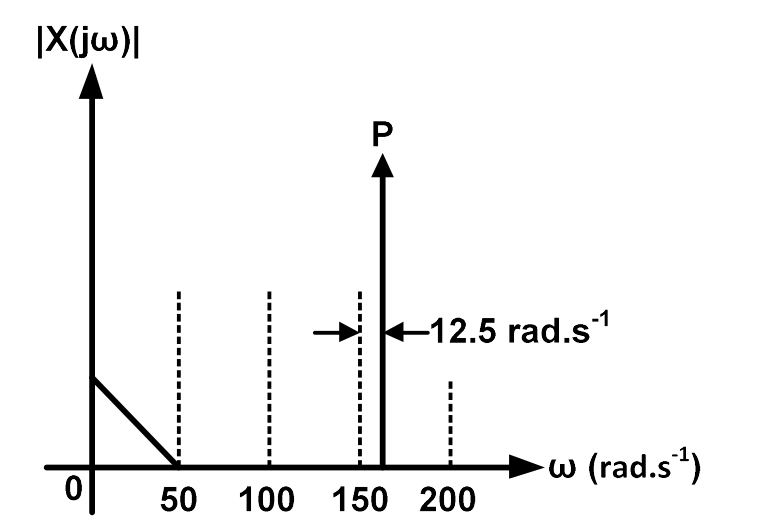
\includegraphics[width=\columnwidth]{2022/BM/14/figs/question.png}
    \caption[short]{Plot of $\abs{X\brak{j\omega}}$}
    \label{fig:2023.bm.14.img1}
\end{figure}

\solution
\fi
\begin{table}[ht]
    \renewcommand\thetable{1}
\begin{tabular}{|c|c|}
    \hline 
    \textbf{Parameter}&\textbf{Description} \\
    \hline
    $w\brak{t}$ & Sampling Function \\
    \hline
	$W\brak{j\omega}$ & Fourier Transform of $w\brak{t}$ \\
    \hline
    $x\brak{t}$ & Input Signal \\
    \hline
    $X\brak{j\omega}$ & Input Signal Frequency Spectrum \\
    \hline
    $x_s\brak{t}$ & Sampled Input Signal \\
    \hline
    $X_s\brak{j\omega}$ & Sampled Signal Frequency Spectrum \\
    \hline
\end{tabular}

\caption{Table of parameters}
\label{Table:1}


\end{table} \\
The sampling function is:
\begin{align}
    w(t) &= \sum_{k = -\infty}^{\infty}\delta\brak{t - \frac{2\pi k}{100}} \\
    W(j\omega) &= 100\sum_{k = -\infty}^{\infty}\delta\brak{j\brak{\omega - 100k}}
\end{align}
then the sampled function: 
\begin{align}
    x_s\brak{t} &= x\brak{t}w\brak{t} \\
    X_s\brak{j\omega} &= X\brak{j\omega} * W\brak{j\omega} \\
    X_s\brak{j\omega} &= \int_{-\infty}^{\infty}X\brak{j\theta}W\brak{j\brak{\omega - \theta}}d\theta \\
    X_s\brak{j\omega} &= 100\sum_{k = -\infty}^{\infty}\int_{-\infty}^{\infty}X\brak{j\theta}\delta\brak{j\brak{\omega - 100k - \theta}}d\theta \\
    X_s\brak{j\omega} &= 100\sum_{k = -\infty}^{\infty}X\brak{j\brak{\omega - 100k}} 
\end{align}
Thus, The down sampled point is at:
\begin{align}
    \omega &= \abs{162.5 - 100k}
\end{align}
where $k$ is the nearest integer to $\frac{162.5}{100}$, which is 2\\
Thus,
\begin{align}
    \omega = 37.5\,rad\,s^{-1}
\end{align}

\begin{figure}[h!]
    \renewcommand\thefigure{2}
    \centering
    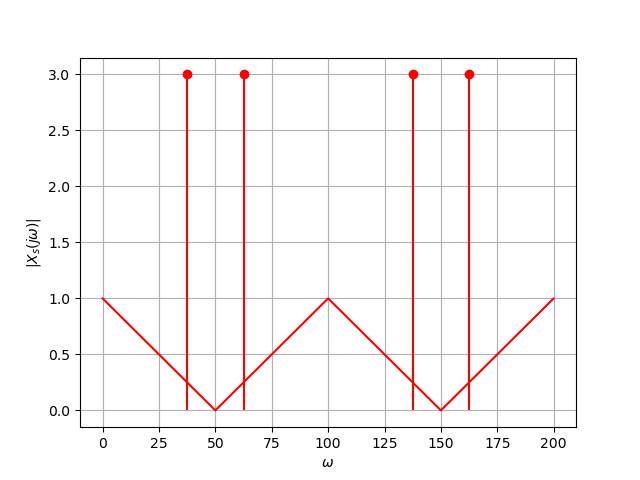
\includegraphics[width=\columnwidth]{2022/BM/14/figs/X_s.png}
    \caption[short]{Plot of $\abs{X_s\brak{j\omega}}$}
    \label{fig:2023.bm.14.img2}
\end{figure}

%\end{document}

\pagebreak
\item Two discrete-time linear time-invarient systems with impulse responses $h_1[n]=\delta[n-1]+\delta[n+1]$ and $h_2[n]=\delta[n]+\delta[n-1]$ are connected in cascade, where $\delta[n]$ is the Kronecker delta. The impulse response of the cascaded system is   \\
\begin{enumerate}[label=(\alph*)]
    \item $\delta[n-2]+\delta[n+1]$
    \item $\delta[n-1]\delta[n]+\delta[n+1]\delta[n-1]$
    \item $\delta[n-2]+\delta[n-1]+\delta[n]+\delta[n+1]$
    \item $\delta[n]\delta[n-1]+\delta[n-2]\delta[n+1]$
\end{enumerate} \hfill(GATE 2021 EE)\\
\solution
\input{2021/EE/7/gate7.tex}
\pagebreak
\item Consider a superheterodyne receiver tuned to 600 kHz. If the local oscillator feeds a 1000 kHz signal to the mixer, the image frequency (in integer) is \underline{\hspace{1cm}} kHz.
\hfill(GATE EC 2021)\\
\solution
\iffalse
\documentclass[journal,12pt,onecolumn]{IEEEtran}
\usepackage{cite}
\usepackage{amsmath,amssymb,amsfonts,amsthm}
\usepackage{algorithmic}
\usepackage{graphicx}
\usepackage{textcomp}
\usepackage{xcolor}
\usepackage{txfonts}
\usepackage{listings}
\usepackage{enumitem}
\usepackage{mathtools}
\usepackage{gensymb}
\usepackage{comment}
\usepackage[breaklinks=true]{hyperref}
\usepackage{tkz-euclide}
\usepackage{listings}
\usepackage{gvv}
\def\inputGnumericTable{}
\usepackage[latin1]{inputenc}
\usepackage{color}
\usepackage{array}
\usepackage{longtable}
\usepackage{calc}
\usepackage{multirow}
\usepackage{hhline}
\usepackage{ifthen}
\usepackage{lscape}

\newtheorem{theorem}{Theorem}[section]
\newtheorem{problem}{Problem}
\newtheorem{proposition}{Proposition}[section]
\newtheorem{lemma}{Lemma}[section]
\newtheorem{corollary}[theorem]{Corollary}
\newtheorem{example}{Example}[section]
\newtheorem{definition}[problem]{Definition}
\newcommand{\BEQA}{\begin{eqnarray}}
    \newcommand{\EEQA}{\end{eqnarray}}
\newcommand{\define}{\stackrel{\triangle}{=}}
\theoremstyle{remark}
\newtheorem{rem}{Remark}

\begin{document}
    
    \bibliographystyle{IEEEtran}
    \vspace{3cm}
    
    \title{Gate 2022 EC Q50}
    \author{EE23BTECH11212 - Manugunta Meghana Sai$^{*}$% <-this % stops a space
    }
    \maketitle
    \bigskip
    
    \renewcommand{\thefigure}{\theenumi}
    \renewcommand{\thetable}{\theenumi}
    
    \vspace{3cm}
    \textbf{Gate 2022 EC Q50} 
    
    Two linear time-invariant systems with transfer functions 
    \begin{align*}
    G_{1}\brak{s} = \frac{10}{s^{2} + s + 1} 
    \end{align*}
    and
    \begin{align*}
    G_{2}\brak{s} = \frac{10}{s^{2}+s\sqrt{10} +10}
    \end{align*}
    have unit step responses $y_{1}\brak{t}$ and $y_{2}\brak{t}$, respectively. Which of the following statements is/are true?
    \begin{enumerate}
    \item $y_{1}\brak{t}$ and $y_{2}\brak{t}$ have the same percentage peak overshoot.\\
    \item $y_{1}\brak{t}$ and $y_{2}\brak{t}$ have the same steady state values.\\
    \item $y_{1}\brak{t}$ and $y_{2}\brak{t}$ have the same damped frequency of oscillation.\\
    \item $y_{1}\brak{t}$ and $y_{2}\brak{t}$ have the same $2\%$ settling time.\\
    \end{enumerate}
    \solution
    \fi
    \begin{table}[h!]
 	\centering
 	\resizebox{6 cm}{!}{
 		\begin{tabular}{|c|c|c|}
	\hline
	\textbf{Parameter} &  \textbf{Description} & \textbf{value}\\[6pt]
	\hline
	$X_{1}\brak{s}$ & input & $\frac{1}{s}$ \\[6pt]
	\hline
	$X_{2}\brak{s}$ & input & $\frac{1}{s}$ \\[6pt]
	\hline
	$G_{1}\brak{s}$ & transfer function & $\frac{10}{s^{2} + s + 1} $ \\[6pt]
	\hline
	$G_{2}\brak{s}$ & transfer function & $\frac{10}{s^{2}+s\sqrt{10} +10} $ \\[6pt]
	\hline
	$y_{1}\brak{t}$ & unit step response & $-$\\[6pt]
	\hline
	$y_{2}\brak{t}$ & unit step response & $-$\\[6pt]
	\hline
	$\omega_{n}$ & natural frequency & $-$\\[6pt]
	\hline
	$\zeta$ & damping ratio & $-$\\[6pt]
	\hline 
	
\end{tabular}

 	}
 	\caption{Given Parameters}
 	\label{tab:msmECgate50tab1}
     \end{table} 
    The general second-order transfer function is given by:
    \begin{align}
    G\brak{s} = \frac{\omega_n^2}{s^2 + 2\zeta\omega_n s + \omega_n^2}
    \end{align}
    After comparing the coefficients of $G_{1}\brak{s}$ and $G_{2}\brak{s}$,
    \begin{table}[h!]
 	\centering
 	\resizebox{6 cm}{!}{
 		\begin{tabular}{|c|c|c|}
	\hline
	\textbf{Tranfer function} &  $\omega_{n}$ & $\zeta$\\[6pt]
	\hline
	$G_{1}\brak{s}$ & $1$ & $\frac{1}{2}$ \\[6pt]
	\hline
	$G_{1}\brak{s}$ & $\sqrt{10}$ & $\frac{1}{2}$ \\[6pt]
	\hline
\end{tabular}

 	}
 	\caption{Given Parameters}
 	\label{tab:msmECgate50tab2}
     \end{table} 
    as $\zeta = \frac{1}{2}$ is less than 1, the system is underdamped.
    \begin{align}
    Y\brak{s} &= X\brak{s} G\brak{s}\\
    &= \frac{1}{s} \brak{\frac{\omega_n^2}{s^2 + 2\zeta\omega_n s + \omega_n^2}}  
    \end{align}
    Applying inverse laplace transform,
    \begin{equation}
    y(t) = 1 - \frac{e^{-\zeta \omega_n t}}{1 - \zeta^2} \sin(\omega_d t + \phi)
    \label{eq:EC50msm}
    \end{equation}
    where $\omega_{d}$ is the damped frequency of oscillation.
    \begin{equation}
    \omega_{d} = \omega_{n}\sqrt{1 - {\zeta}^2}
    \label{eq:EC50msm2eq}
    \end{equation}
    The percentage peak overshoot $\brak{PO}$:
    \begin{equation}
    PO = \left( \frac{y_{\text{max}} - y_{\text{ss}}}{y_{\text{ss}}} \right) \times 100\%
    \label{eq:EC50msm1eq}
    \end{equation}
    $y_{\text{max}}$ is obtained by differentiating~\eqref{eq:EC50msm} with respect to time and equating it to zero, substituting the value in~\eqref{eq:EC50msm},
    \begin{align}
    y_{\text{max}} = 1 + \frac{1}{\sqrt{1-{\zeta}^2}}
    \end{align}
    $y_{\text{ss}}$ is obtained by final value theorem,
    \begin{align}
    y_{\text{ss}} &= \lim_{{s \to 0}} sY(s)\\
    &= \lim_{{s \to 0}} s\frac{\omega_n^2}{s^2 + 2\zeta\omega_n s + \omega_n^2} \frac{1}{s}\\
    &= 1
    \end{align} 
    Substituting the values of $y_{\text{max}}$ and $y_{\text{ss}}$ in~\eqref{eq:EC50msm1eq}, 
    \begin{align}
    PO = \frac{1}{\sqrt{1-{\zeta}^2}} \times 100\%
    \end{align}
    $y_{1}\brak{t}$ and $y_{2}\brak{t}$ have same $\zeta$, they have same percentage peak overshoot.So, option $\brak{1}$ is correct.\\
    The steady state value of $y\brak{t}$ is given by final value theorem:
    \begin{align}
    y_{1ss} &= \lim_{{s \to 0}} sY_{1}(s)\\
    &= \lim_{{s \to 0}} s \frac{10}{s^{2} + s + 1}  \frac{1}{s}\\
    &= 10\\
    y_{2ss} &= \lim_{{s \to 0}} sY_{2}(s)\\
    &= \lim_{{s \to 0}} s \frac{10}{s^{2}+s\sqrt{10} +10}  \frac{1}{s}\\
    &= 1
    \end{align} 
    as both the unit step responses have different steady state values, option $\brak{2}$ is incorrect.\\
    From~\eqref{eq:EC50msm1eq}, as $\omega_{n}$ is different for $y_{1}\brak{t}$ and $y_{2}\brak{t}$, they have different damped frequency of oscillation. Hence option $\brak{3}$ is incorrect.\\
    Settling time $T_s$:
    \begin{align}
    T_s = \frac{4}{\zeta \omega_n}
    \end{align}
    As, $\omega_{n}$ is different for $y_{1}\brak{t}$ and $y_{2}\brak{t}$, they have different $2\%$ settling time, Hence option $\brak{4}$ is incorrect.\\
    So, only option $\brak{1}$ is correct.   
%\end{document}


\pagebreak
\item For a unit step input $u[n]$, a discrete-time LTI system produces an output signal $(2\delta[n+1]+\delta[n]+\delta[n-1])$. Let $y[n]$ be the output of the system for an input $\brak{\brak{\frac{1}{2}^n}u[n]}$. The value of $y[0]$ is:  \hfill(GATE EC 2021) \\
\solution
\iffalse
\let\negmedspace\undefined
\let\negthickspace\undefined
\documentclass[journal,12pt,twocolumn]{IEEEtran}
\usepackage{cite}
\usepackage{amsmath,amssymb,amsfonts,amsthm}
\usepackage{algorithmic}
\usepackage{graphicx}
\usepackage{textcomp}
\usepackage{xcolor}
\usepackage{txfonts}
\usepackage{listings}
\usepackage{enumitem}
\usepackage{mathtools}
\usepackage{gensymb}
\usepackage{comment}
\usepackage[breaklinks=true]{hyperref}
\usepackage{tkz-euclide} 
\usepackage{listings}
\usepackage{gvv}                                        
\def\inputGnumericTable{}                                 
\usepackage[latin1]{inputenc}                                
\usepackage{color}                                            
\usepackage{array}                                            
\usepackage{longtable}                                       
\usepackage{calc}                                             
\usepackage{multirow}                                         
\usepackage{hhline}                                           
\usepackage{ifthen}                                           
\usepackage{lscape}

\newtheorem{theorem}{Theorem}[section]
\newtheorem{problem}{Problem}
\newtheorem{proposition}{Proposition}[section]
\newtheorem{lemma}{Lemma}[section]
\newtheorem{corollary}[theorem]{Corollary}
\newtheorem{example}{Example}[section]
\newtheorem{definition}[problem]{Definition}
\newcommand{\BEQA}{\begin{eqnarray}}
\newcommand{\EEQA}{\end{eqnarray}}
\newcommand{\define}{\stackrel{\triangle}{=}}
\theoremstyle{remark}
\newtheorem{rem}{Remark}

\usepackage{graphicx}
\graphicspath{ {./Downloads/} }
\begin{document}

\bibliographystyle{IEEEtran}
\vspace{3cm}

\title{GATE 2021}
\author{EE22BTECH11060 - TEJAVATH KUSHAL$^{*}$% <-this % stops a space
}
\maketitle
\newpage
\bigskip

\renewcommand{\thefigure}{\theenumi}
\renewcommand{\thetable}{\theenumi}


\maketitle
\noindent \textbf{Q.40} : 
For a unit step input $u[n]$, a discrete-time LTI system produces an output signal $(2\delta[n+1]+\delta[n]+\delta[n-1])$. Let $y[n]$ be the output of the system for an input $\brak{\brak{\frac{1}{2}^n}u[n]}$. The value of $y[0]$ is:
\begin{flushright}
\brak{\text{GATE 2021 EC}}
\end{flushright}

\noindent \textbf{Ans.}
\fi

\begin{table}[h]
  \centering
\begin{tabular}{|c|c|}
        \hline
        \textbf{Input} & \textbf{Output} \\
        \hline
        $u[n]$ & $s\brak{n}=2\delta[n+1]+\delta[n]+\delta[n-1]$ \\ 
	\hline
	$\brak{\frac{1}{2}}^nu[n]$ & $y[n]$  \\ 
        \hline
\end{tabular}
\caption{Input-Output parameter table}
\label{tab:gate.2023.ec.40.1}





\end{table}

\noindent For impulse response
\begin{align}
h\brak{n}&=s\brak{n}-s\brak{n-1}\\
\notag h\brak{n} &=2\delta\brak{n+1}+\delta\brak{n}+\delta\brak{n-1}-2\delta\brak{n} \\
&~~~~~~~~~~~~~~-\delta\brak{n-1}-\delta\brak{n-1-1}\\
\implies h\brak{n} &=2\delta\brak{n+1}-\delta\brak{n}-\delta\brak{n-2}
\end{align}
\text{For input }$x\brak{n}=\brak{\frac{1}{2}}^nu\brak{n}$
\begin{align}
y\brak{n} &= x\brak{n}*h\brak{n}\\
 &= x\brak{n}*[2\delta\brak{n+1}-\delta\brak{n}-\delta\brak{n-2}]\\
 &= 2x\brak{n+1}-x\brak{n}-x\brak{n-2}\\
\notag  &=2\brak{\frac{1}{2}}^{n+1}u\brak{n+1}-\brak{\frac{1}{2}}^nu\brak{n}\\
&~~~~~~~~~~~~~~~~~~~-\brak{\frac{1}{2}}^{n-2}u\brak{n-2}\\
\implies y\brak{0} &=0
\end{align}\\
\pagebreak
\begin{figure}[h]
    %\caption{ Plot of $y\brak{n}$ v/s n}
    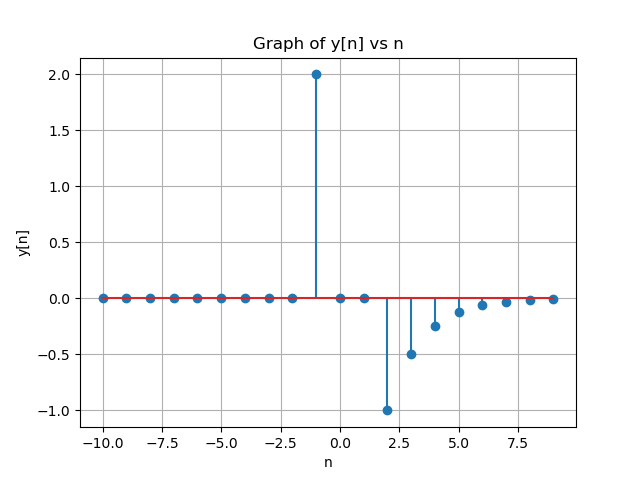
\includegraphics[width=0.5\textwidth]{2021/EC/40/figs/y(n) vs n.png}\label{fig:stem plot}
    \caption{Plot of $y\brak{n}$ v/s n}
\end{figure}






\pagebreak
\end{enumerate}
